%! Author = enzo
%! Date = 19-04-23

% Preamble
\documentclass[../main.tex]{subfiles}

%%puedo crear comandos que solo sirven en este archivo.
%%pero los comando definidos en el main afectan este archivo.
%
%%codigo para imprimir dibujos:
%\newcounter{numeroCapituloApendice}%ponemos un contador que empieza en 0 y que cuenta el número de clase
%
%%creamos una clase, i.e. ponemos un aseccion con el numero de clase y con un argumento obligatorio \Clase{argumento obligatorio} que es la fecha de la clase, por ejemplo 13/03/23.
%\newenvironment{Capitulo}[1]{
%	\stepcounter{numeroCapituloApendice}
%    \chapter{Capitulo \thenumeroCapituloApendice: #1}
%}{}
%
%%%%%%%%%%%%%%%%%%%%%%%%%%%%%%%
%%Cada dibujo se puede automatizar:
%%1) necesitamos el archivo "Dibujo n.png" en la carpeta "Clase m", donde $n$ es el número del dibujo y $m$ es el número de la clase.
%
%\newcounter{numeroDibujoApendice}[numeroCapituloApendice]
%
%%\renewcommand\thefigure{\thechapter.\arabic{figure}}
%
%%el comando Dibujo tiene dos inputs \Dibujo{input 1}{input 2}, el primer input es el número de dibujo y el segundo es el caption de la figura.
%\NewDocumentCommand{\DibujoApendice}{O{0.8} m}{
%\stepcounter{numeroDibujoApendice}
%\begin{center}
%\includegraphics[width=#1\columnwidth]{"./Apendice/Figuras/Capitulo \thenumeroCapituloApendice /Dibujo \thenumeroDibujoApendice .pdf"}
%\captionof{figure}{#2}
%\end{center}
%}
%



% Document
\begin{document}



\appendix

\chapter{Primera parte de la materia (primer capítulo del Diestel)}

\section[]{Un poco de álgebra lineal}

Sea $G = (V,E)$ un grafo con $n$ vértices y $m$ aristas, digamos $V = \{v_1,\ldots,v_n\}$ y $E = \{e_1,\ldots,e_m\}$.

\begin{definition}
El \textbf{espacio de vértices} $\mathcal{V} (G)$ de $G$, es el $\mathbb{F}_2$-espacio vectorial de todas las funciones $V \rightarrow \mathbb{F}_2$.
\end{definition}
Todo elemento de $\mathcal{V} (G)$ corresponde naturalmente con un subconjunto de $V$, más precisamente con la preimagen de $1$, y más aún todo subconjunto de $V$ se representa de manera única de esta manera por su función indicadora. Con lo cual, podemos identificar a $\mathcal{V} (G)$ con el conjunto de subconjuntos de $V$, i.e. $2^V$; así tenemos un espacio vectorial de los subconjuntos de $V$: $U + U' = U \Delta U'$ es la diferencia simétrica! y $U = -U$. El cero en este espacio vectorial corresponde con el subconjunto vacío $\emptyset \subset V$. Notar que $\{ \{ v_1 \}, \ldots, \{ v_n\} \}$ es una base de $\mathcal{V} (G)$, llamada la \textbf{base standard}; tenemos entonces que $\dim \mathcal{V} (G) = n$.


\begin{definition}
Análogamente, podemos definir el \textbf{espacio de aristas} $\mathcal{E} (G)$ de $G$, más precisamente, el $\mathbb{F}_2$-espacio vectorial de funciones $E \rightarrow \mathbb{F}_2$.
\end{definition}
Nuevamente, los elementos de $\mathcal{E} (G)$ se corressponden con subconjuntos de $E$: tomamos la preimagen de $1$. En este caso, la suma de vectores es la diferencia simétrica de conjuntos de aristas, y el conjunto vacío $\emptyset \subset E$ corresponde con el cero, además $F = -F$ para todo $F \subset E$. La \textbf{base standard} es $\{ \{e_1\},\ldots \{e_m\} \}$, luego $\dim \mathcal{E} (G) = m$.

Dados $F,F' \in \mathcal{E} (G)$, vistos como funciones, podemos definir:
\[
    \langle F, F' \rangle := \sum_{e \in E} F (e) F'(e) \in \mathbb{F}_2.
\]
Esta cantidad es cero si y solo si $F$ y $F'$ tienen una cantidad par de aristas en común, i.e $\abs{F \cap F'} \equiv 0 \mod 2$; en particular ciertamente puede suceder que $\langle F , F \rangle = 0$ con $F \neq \emptyset$. De todas formas, es simétrico y $\mathbb{F}_2$-bilineal.
De manera la manera usual, para cualquier subespacio $\mathcal{F} \subset \mathcal{E}(G)$, podemos definir el subespacio ortogonal:
\[
    \mathcal{F}^\perp := \Set{D \in \mathcal{E}(G) | \langle F , D \rangle = 0, \\ \forall F \in \mathcal{F}}.
\]
Que es un subespacio. Se tiene que
$$
\dim \mathcal{F} + \dim \mathcal{F}^\perp = m.
$$
Pues se sigue de la demostración standard, ya que este producto es \textit{no degenerado}, es decír el morfismo de espacios vectoriales $F \mapsto \langle \cdot, F \rangle$ es inyectivo, luego la ecuación se sigue de álgebra lineal (estudiando el espacio dual).

\begin{definition}
El \textbf{espacio de ciclos} $\mathcal{C} = \mathcal{C}(G)$ es el subespacio de $\mathcal{E}(G)$ generado por todos los ciclos de $G$ (por sus aristas). La dimensión de este espacio se lo llama a veces \textbf{número ciclomático} de $G$.
\end{definition}

\begin{proposition}
Las siguientes afiirmacaiones son equivalentes para conjuntos de aristas $D \subset E$:
\begin{enumerate}[1.]
\item $D \in \mathcal{C} (G)$;
\item $D$ es una unión (posiblemente vacía) disjunta de ciclos en $G$;
\item Todos los grados de los vértices de $(V,D)$ son pares.
\end{enumerate}
\end{proposition}
\begin{proof}
Como los ciclos tienen grados pares y tomar diferencia simétrica preserva esta propiedad, luego 1. implica 3. por inducción en la cantidad de ciclos que generan $D$ con la suma. Que 3. implica 2. se sigue por inducción en $\abs D$: si $D \neq \emptyset$ entonces $(V,D)$ contiene un ciclo por la Proposición \ref{proposition:todo grafo tiene un camino de largo >= delta y ciclo de largo >= delta +1}, borrando las aristas de $C$ podemos proceder inductivamente pues los vértices siguen teniendo grado par. Finalmente la implicación 2. $\Rightarrow$ 1. es inmediata de la definición de $\mathcal{C}(G)$.
\end{proof}



\begin{definition}
Un conjunto $F$ de aristas se dice un \textbf{corte}\footnote{No vamos a incluir el caso de particiones vacías. Luego la única manera de que el conjunto vacío de aristas sea un corte es que el grafo subyacente sea disconexo.}
 de $G$ si existe una partición $\{V_1,V_2\}$ de $V$ tal que $F = E(V_1,V_2)$. Decimos que las aristas de $F$ \textbf{cortan} esta partición. Los conjuntos $V_1,V_2$ son los \textbf{lados} del corte. A un corte no vacío minimal lo llamamos \textbf{enlace}.
\end{definition}

\begin{proposition}
Junto con el conjunto vacío $\emptyset$, los cortes en $G$ forman un subespacio $\mathcal B = \mathcal B ( G) \subset \mathcal{E}(G)$. Este espacio está generado por los cortes de la forma $E(v)$ ( es decir los conjuntos de aristas incidentes a un vértice).
\end{proposition}
\begin{proof}
Sea $\mathcal B$ el subespacio generado por los cortes de la forma $E(v)$ en $\mathcal{E} (G)$. Todo corte de $G$, con partición $\{ V_1 , V_2 \}$, coincide con $\sum_{v \in V_1} E(v)$ y por lo tanto está en $\mathcal{B}$. En efecto, el conjunto $\sum_{v \in V_1} E(v)$ es la diferencia simétrica de los conjuntos $E(v)$, i.e. las aristas que están en algún $E(v), v  \in V_1$ pero no en todos, es decir, las aristas que inciden en un vértice de $V_1$ y que su otro extremo no puede estár en $V_1$, es decir tiene que estár en $V_2$. Recíprocamente, todo conjunto $\sum_{u \in U}E(u) \in \mathcal{B}$ es vacío, por ejemplo si $U \in \{ \emptyset , V \}$, o es el corte $E(U, V \setminus U)$ (mismo razonamiento de antes).
\end{proof}

\begin{definition}
El espacio $\mathcal{B} (G)$ es el \textbf{espacio de cortes}, o el \textbf{espacio de enlaces} de $G$.
\end{definition}

\begin{obs}
Los enlaces son para $\mathcal B$, lo que son los ciclos para $\mathcal C$: elementos minimales no vacíos.

Si $G$ es conexo, entonces los enlaces son justamente sus cortes minimales: un corte en un grafo conexo es minimal si y solo si ambos lados de la partición inducen subgrafos conexos. En efecto, por un lado, dados un corte minimal con bipartición $\{V_1,V_2\}$ induce subgrafos conexos $G[V_1],G[V_2]$, pues de lo contrario eligiendo un vértice $v_1 \in V_1$ aislado en $G[V_1]$, se sigue que el corte $E(V_1 \setminus \{v_1 \}, V_2 \cup \{ v_1 \})$ pierde todas la $V_1,V_2$ aristas incidentes en $v_1$ ($G$ es conexo), contradiciendo minimalidad; por otro lado, un corte con bipartición $\{V_1,V_2\}$ de conjuntos de vértices que inducen subgrafos conexos tiene que ser minimal, de lo contrario es que se le pueden quitar aristas y sigue siendo un corte, luego es porque uno de los subgrafos inducidos no era conexo. Ahora, si $G$ es disconexo, luego sus enlases sson los cortes minimales de sus componentes conexas, pues unir cortes de cada componente conexa sigue dando un corte (y por lo tanto un corte no es minimal a menos que esté contenido en una componente).
\end{obs}

\begin{lemma}
Todo corte es la unión disjunta de enlaces.
\end{lemma}
\begin{proof}
Haremos inducción en el tamaño del corte $F$ a considerar. Para $F = \emptyset$ no hay nada que probar. Si $F \neq \emptyset$, y no es un enlace, luego contiene propiamente a algún corte $F'$. Por la proposición anterior, la suma de cortes es un corte (forman un subespacio), es decir $F \setminus F' = F + F'$ es un corte más chico no vacío. Por inducción tenemos que $F'$ y $F \setminus F'$ son ambos unión disjunta de enlaces, y por lo tanto $F$ también.
\end{proof}

\begin{exercise}
Hallar una base de $\mathcal{B}(G)$ dada por conjuntos de aristas de la forma $E(v)$.
\end{exercise}
\begin{solution}
Sabemos que los $E(v), v \in V(G)$ generan $\mathcal{B}(G)$; afirmamos que si $G$ es conexo, entonces para todo $w \in V(G)$ el siguiente conjunto forma una base del subespacio de cortes:
$$
\{ E(v) \}_{v \in V(G) \setminus \{w\}}.
$$
En efecto, el conjunto de generadores de $\mathcal{B}(G)$ es linealmente dependiente porque $\sum_{v \in V(G)} E(v) = \emptyset$, pero si quitamos cualquier vértice se vuelve linealmente independiente, pues que sea linealmente dependiente equivale a que existe un subconjunto $S \subsetneq V(G)$ no vacío tal que
$$
\emptyset = \sum_{v \in S} E(v) = E(S, V(G) \setminus S),
$$
que es imposible si $G$ es conexo.

En general, si $G$ no es conexo escribimos $G = \bigsqcup_i C_i$, donde $C_i$ son sus componentes conexas, luego una base de $\mathcal{B}(G)$ es la unión de las bases de $\mathcal{B}(G_i)$, pues podemos hacer el abuso de notación $\mathcal{B}(G) = \bigoplus_i \mathcal{B}(G_i)$.
\end{solution}



\begin{corollary}
Se sigue que
$$
\dim \mathcal{B} (G) = \sum_{C \text{ componente de $G$}} (\abs{C} -1) = \abs{G} -  \# \{\text{componentes de $G$}\}.
$$
En particular si $G$ es conexo,
\[
    \dim \mathcal{B} (G) = \abs G -1.
\]
\end{corollary}

\begin{exercise}
Construir de manera explícita la partición en enlaces de un corte: sea $F$ un corte en $G$, con partición $\{V_1, V_2\}$. Para $i = 1,2$ escribamos $C_1^i, \ldots, C^i_{k(i)}$ a las componentes conexas de $G[V_i]$. Usar los $C_j^i$ para definir los enlaces que forman una unión disjunta para $F$.
\end{exercise}
\begin{solution}
Vamos a considerar el caso $G$ conexo, pues el caso disconexo directamente escribimos a un corte como la unión disjunta de sus aristas en cada componente. Ahora, si $G$ es conexo consideremos los conjuntos de aristas
$$
E(C_i^1 \cup \bigcup_{C_j^2 \cap N (C_i^1) \neq \emptyset} C_j^2, \bigcup_{C_j^2 \cap N(C_i^1) = \emptyset} C_j^2 \cup \bigcup_{C_k^1 \neq C_i^1} C_{k}^1),
$$
para todo $1 \leq i \leq k(1)$ fijo. Hay que verificar que estos son disjuntos entre si, y su unión da $E(V_1,V_2)$, y además que son enlaces (basta ver que su partición induce subgrafos conexos). En efecto, $E(V_1,V_2)$ está claramente contenido en su unión; recíprocamente, las aristas de $E(C_i^1 \cup N (C_i^1)\cap V_2, *)$ están en $E(V_1,V_2)$ pues hay dos posibilidades: o la arista está en $E(C_i^1, C_j^2)$ con $C_j^2 \cap N (C_i^1) = \emptyset$ o está en $E(C_j^2,C_{i'}^1)$. Por contrucción son enlaces porque cada parte de la partición es un subgrafo inducido conexo, pues la parte $\bigcup_{C_j^2 \cap N(C_i^1) = \emptyset} C_j^2 \cup \bigcup_{C_k^1 \neq C_i^1} C_{k}^1$ tiene que ser conexa porque $G$ lo es y las $C_j^i$ con $i$ fijo no están conectadas entre sí porque son las componentes de $V_i$. Finalmente, tienen que ser claramente disjuntas.
\end{solution}

\begin{theorem}
El espacio de ciclos $\mathcal{C}(G)$ y el espacio de cortes $\mathcal{B}(G)$ de cualquier grafo satisfacen
\[
    \mathcal C = \mathcal B^{perp} \quad \text{y} \quad \mathcal B = \mathcal C^{\perp}.
\]
\end{theorem}
\begin{proof}
Consideremos un grafo $G = (V,E)$. Claramente todo ciclo en $G$ tiene un número par de aristas en cada corte, luego los ciclos son ortogonales a los cortes, es decir
$$
\mathcal{C}(B) \subset \mathcal{B}(G)^\perp \quad \text{y} \quad \mathcal(B)(G)  \subset \mathcal{C}(G)^\perp.
$$

Para probar $\mathcal{B}(G)^\perp \subset \mathcal C$ hay que usar la anteúltima proposición que caracteriza los vectores del subespacio de ciclos, es decir $F \not \in \mathcal{C}(G)$ si y solo si tiene un vértice incidente con un número impar de aristas en $F$. Luego $\langle E(v), F \rangle = 1$, entonces como $E(v) \in \mathcal{B}(G)$ se sigue que $F \not \in \mathcal{B}(G)^\perp$. Esto termina de probar que $\mathcal C = \mathcal B ^\perp$ en $G$.

Finalmente, para probar $\mathcal (G)^\perp \subset \mathcal B (G)$, tomemos $F \in \mathcal C (G)^\perp$. Consideremos el \textit{multigrafo} $H$ obtenido a partir de $G$ luego de contraer las aristas de $E \setminus F$. Todo ciclo en $H$ tiene sus aristas en $F$. Como lo podemos extender a cualquier ciclo en $G$ agergando aristas de $E\setminus F$, entonces el número de aristas del ciclo extendido que están en $F$ (es decir las aristas del ciclo en $H$ original) debe ser par, pues $F \in \mathcal C ^\perp$. Usando la caracterización de grafos bipartitos, tenemos q ue $H$ es bipartito. Su partición induce una partición $(V_1,V_2)$ de $V$ (ya que las aristas que habíamos contraído convierten la bipartición en un corte), tal que $E(V_1,V_2) = F$, i.e. $F \in \mathcal{B}(G)$.
\end{proof}



Consideremos ahaora un grafo conexo $G = (V,E)$ con un árbol generador $T \subset G$. Para toda cuerda $e \in E \setminus E(T)$ existe un único ciclo $C_e$ en $T+e$, que llamaremos el \textbf{ciclo fundamental} de $e$ con respecto a $T$. Similarmente, para toda arista $f \in T$, el bosque tienee exactamente dos componentes (por la caracterización de árbol). El conjunto $D_f \subset E$ de aristas de $G$ entre ambas componentes es un \textit{enlace} (usando una de las propiedades probadas en essta sección, pues ambos lados de la partición son subgrafos inducidos conexos) en $G$, el \textbf{corte fundamental} de $f$ con respecto de $T$.

Notar que $f \in C_e$ si y solo si $e \in D_f$, para todo $e \not \in T$ y $f \in T$. En efecto, por un lado si $e \not \in T$ y $f \in T$, entonces $f \in C_e$ entonces sacar a $f$ de $T$ hace que se parta en dos componentes, que tienen que estar conectada por la cuerda $e$ ya que todo camino entre ambas componentes pasaba por $f$, luego por $C_e$ y cuando quitas una arista de un ciclo los caminos pueden seguir pasando por los vértices de $f$ a través de $e$, i.e. $e \in D_f$. Por otro lado, si $e \in D_f$ entonces el camino $f \cdots e \cdots f$ tiene que ser un ciclo en $G$ porque las aristas de $f \cdots e$ están en una componente y las aristas $e \cdots f$ en otra, así $f \in C_e$. Esto indica una conexión más profunda de dualidad; el siguiente teorema explora un poco este descubrimiento.

\begin{figure}
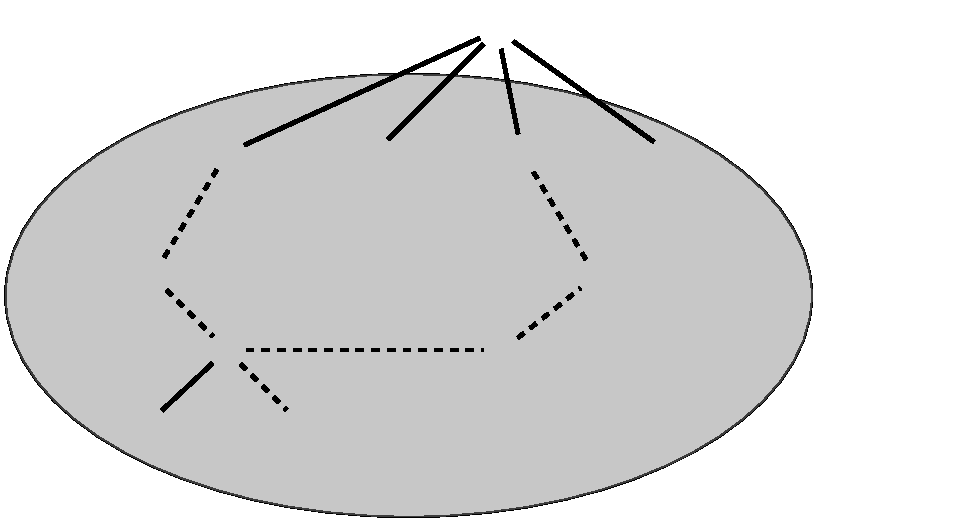
\includegraphics[width=\linewidth]{"./Apendice/Figuras/Capitulo 1/Dibujo 1.pdf"}
\caption{Ejemplo: El ciclo fundamental \red{$C_e$}, y el corte fundamental \blue{$D_f$}.}
\end{figure}


\begin{theorem}
Sea $G$ un grafo conexo con $n$ vértices y $m$ aristas, y sea $T \subset G$ un árbol generador.
\begin{enumerate}[(i)]
\item Los cortes fundamentales y los ciclos fundamentales de $G$ respecto de $T$ forman bases de $\mathcal{B}(G)$ y $\mathcal{C}(G)$, respectivamente.
\item Consecuentemente,
$$
\dim \mathcal{B}(G) = n-1 \quad \text{y} \quad \dim \mathcal{C}(G) = m - n + 1.
$$
\end{enumerate}
\end{theorem}
\begin{proof}
\begin{enumerate}[(i)]
\item Notemos que toda arista $f \in T$ yace en $D_f$, pero ningún otro corte fundamental lo hace (estas son aristas de $T$), mientras que una arista $e \not \in T$ yace en $C_e$ pero no en otro ciclo fundamental (este ciclo está construido con una sola arista fuera de $T$).
Es decir, dados un subconjunto arbitrario de cortes fundamentales $\{ D_{f_1}, \ldots, D_{f_r}\}$, entonces
$$
\sum_{i = 1}^r D_{f_i} \neq \emptyset.
$$
Análogamente, lo mismo sucede para un subconjunto de ciclos sfundamentales $\{ C_{e_1}, \ldots, C_{e_s} \}$.
Con lo cual los cortes fundamentales y los ciclos fundamentales son, respectivamente, conjuntos linealmente independientes en $\mathcal B = \mathcal B (G)$ y $\mathcal C  = \mathcal C (G)$.

Veamos ahora que los ciclos fundamentales generan a un ciclo $C$ arbitrario. Por nuestra observación inicial, $D := C + \sum_{e \in C \setminus T} C_e$, es decir a $C$ le estamos quitando todas las aristas fuera de $T$, es un elemento de $\mathcal C$, que no contiene ningúna arista fuera de $T$, i.e. está contenido en $T$. Pero la Proposición \ref{} los elementos de $\mathcal C$ son unión disjunta de ciclos, pero como $T$ es aciclico, la única opción es que sea el conjunto $\emptyset$. En consecuencia $D = \emptyset$ y en particular $C = \sum_{e \in C \setminus T} C_e$.

Similarmente, todo corte $D$ es la suma de cortes fundamentales. En efecto, el elemento $D + \sum_{f \in D \cap T} D_f$ de $\mathcal B$ no contiene aristas en $T$. Así es, pues si $e \in (E(G) \setminus E(T)) \cap (D + \sum_{f \in D \cap T} D_f)$, entonces por la observación inicial $C_e \cap (D + \sum_{f \in D \cap T} D_f) = \{e\}$ ya que la única arista extra $g$ que podría aparecer debería estar en $T$ pues $C_e$ de lo contrario $g \in C_g \cap C_e$, por otro lado $g$ está en $D$ o en algún $D_f$; por un lado si está en $D$ luego está en un único $D_f$ por la observación inicial, es decir no está en $D + \sum_{f \in D \cap T} D_f$, por otro lado si no oestá en $D$, no puede estar en ningún $D_f$ con $f \in D \cap T$ pues $D_f$ contiene a un único corte fundamental. En resumen, $D + \sum_{f \in D \cap T} D_f$ es vacío. Es decir, $D = \sum_{f \in D \cap T} D_f$.
\item Por un ladod hay $n-1$ cortes fundamentales, pues hay uno por cada arista del arbol generador $T$ de $G$, el cual tiene $n$ vértices (usamos que los grafos conexos de $n$ vértices tienen $n-1$ aristas si y solo si son árboles). Por otro lado, como vimos que $\mathcal C (G) = \mathcal B (G)^\perp$ y que para todo subespacio $V \subset \mathcal \epsilon (G)$ se tiene $\dim V + \dim V^\perp = \dim \mathcal E (G) = m$, se sigue que $\dim \mathcal C (G) = m-n+1$.
\end{enumerate}
\end{proof}


\begin{definition}
    La \textbf{matriz de incidencia} $B = (b_{ij})_{n \times m} \in \mathbb{F}_2^{n\times m}$ de un grafo $G = (V,E)$
    con $V = \{ v_1
    ,\ldots, v_n\}$ y $E = \{e_1,\ldots,e_m\}$ está dada por
    \[
        b_{ij} := \begin{cases}
                    1 & \text{ si $v_i \in e_j$}\\
                    0 & \text{ si no.}
                    \end{cases}
    \]
    Luego las matrices $B$ y $B^t$ definen las transformaciones lineales
    \[
        B : \mathcal E (G) \rightarrow \mathcal V (G) \quad \text{y} \quad B^t \mathcal V (G) \rightarrow \mathcal E (G)
    \]
    definidas respecto de las bases standard.
\end{definition}

\begin{obs}
La transformación $B$ manda conjuntos de aristas $F \subset E$ en al conjunto de vértices incidentes en un número
impar de aristas de $F$. Mientras que $B^t$ manda un conjunto de vértices $U \subset V$ en el lconjunto de aristas
con exactamente un solo extremo en $U$.
\end{obs}

Como consecuencia obtenemos:

\begin{corollary}
\begin{enumerate}[(i)]
\item El núcleo de $B$ es $\mathcal C(G)$.
\item La imagen de $B^t$ es $\mathcal B (G)$.
\end{enumerate}
\end{corollary}
\begin{proof}
\begin{enumerate}[(i)]
\item $C \in \Ker B$ si y solo si todos los vértices de $G$ tienen un número par de aristas incidentes en $C$, es
decir $(G,C)$ tiene todos sus vértices de grado par, lo cual es una definición equivalente de estar en $\mathcal C (G)$.
\item Sea $U \subset V$, entoncces $B^t (U) = F$ el conjunto de aristas con exactamente un extremo en $U$, es decir, $F = E(U, V \setminus U)$ es un corte.
\end{enumerate}
\end{proof}


\begin{definition}
La \textbf{matriz de adyasencia} $A = (a_{ij})_{n \times n} \in \mathbb{F}_2^{n \times n}$ de $G$ está dada por
\[
    a_{ij} := \begin{cases}
            1 & \text{ si $v_{i} v_j \in E$}\\
            0 & \text{ si no.}
                \end{cases}
\]
\end{definition}

\begin{obs}
Esta matriz es simétrica. Además, se puede ver como una transformación lineal $A : \mathcal V (G) \rightarrow \mathcal V (G)$, que manda subconjuntos de vértices $U \subset V$ al conjunto de vértices con un número impar de vecinos en $U$.
\end{obs}

Denotemos por $D$ a la matriz \textit{real} diagonal $(d_{ij})_{n \times n} \in \reals^{n \times n}$ con $d_{ii} = d(
v_i)$. Nuestra última proposición establece una conexión de $A$ y $B$ vistos como matrices reales:

\begin{proposition}
$$
B \cdot B^t = A + D.
$$
\end{proposition}
\begin{proof}
La cuenta se tiene que hacer entre matrices reales, la cual una cuenta muy elemental.
\end{proof}

Notar que la misma ecuación sigue valiendo módulo $2$.


\section[]{Otras nociones sobre grafos}

\begin{definition}
Un \textbf{hipergrafo} es un par $(V,E)$ de conjuntos disjuntos, donde los elementos de $E$ son subconjuntos no vac
íos (de cualquier cardinalidad) de $V$. Con lo cual, los grafos son un caso particulara de los hipergafos.
\end{definition}

\begin{definition}
    Un \textbf{grafo dirigido} o \textbf{digrafo} es un par $(V,E)$ de conjuntos disjuntos de vértices y aristass,
    junto con dos funciones $\operatorname{init}: E \rightarrow V$ y $\operatorname{ter} : E \rightarrow V$ que
    mandan una arista $e$ en un \textbf{vértice inicial} $\operatorname{init}(e)$ y en un \textbf{vérticce terminal} $\operatorname{ter}(e)$. La arista $e$ se dice \textbf{dirigida desde $\operatorname{init}(e)$ hasta $\operatorname{ter}(e)$}.
\end{definition}
Notar que un grafo dirigido puede tenenr varias aristas entre dos vértices $x,y$. Estas aristas se llaman \textbf{
aristas múltiples}; si tienen la misma dirección, digamos de $x$ a $y$, se dicen \textbf{paralelas}. Si $\operatorname{init}(e) = \operatorname{ter}(e)$, decimos que $e$ es un \textbf{bucle}.

Un grafo dirigido $D$ es una \textbf{orientación} de un grafo (sin dirigir) $G$ si $V(D) = V(G) $ y $E (D) = E(G)$, y
 además $\{ \operatorname{init}(e), \operatorname{ter}(e)= \{x,y\}$ para toda ariwstas $e = xy$. Intuitivamente, este \textbf{grafo orientado} surge de un grafo sin dirigir simplemente luego de darle una orientación a cada arista de $G$, desde uno de sus extremos hasta el otro. En particular, los grafos orientados son grafos dirigidos sin bucles ni aristas multiples.

 \begin{definition}
     Un \textbf{multigrafo} es un par $(V,E)$ de conjuntos disjuntos de vértices y aristas con una función $E \rightarrow V \cup [V]^2$ que le asigna a cada arista uno o dos vértices a sus extremos.
 \end{definition}
Por lo tanto, los multigrafos pueden tener bucles y aristas multiples: podemos pensar a los multigrafos como grafos
dirigidos, donde las direcciones de sus aristas fueron eliminadas. Para expresar que $x$ e $y$ son los extremos de
una arista $e$, escribimos $e = xy$, sin embargo esta escritura no siempre es única!

Un grafo es entonces un multigrafo sin bucles ni aristas múltiples. De manera sorprendente, a veces probar un teorema
 para grafos es más díficil que probar para multigrafos. Más aún, existen áreas de la teoría de grafos donde los
 multigrafos surgen de manera más natural que los grafos, y donde restringirse a estos últimos resulta artificial y
 más complicado (por ejemplo dualidad de planos). Para multigrafos usaremos la misma terminología que vimos para
 grafos, pues estas definiciónes se trasladan de manera obvia. Por ejemplo, ver la Figura \ref{Fig 2 - Apendice 1}.

 \begin{center}
 \begin{figure}
    \includegraphics[width=0.7\linewidth]{"./Apendice/Figuras/Capitulo
    1/Dibujo 2"}
    \caption{Contración de la arista $e$ en un multigrafo $G$.}
\end{figure}
\label{Fig 2 - Apendice 1}
\end{center}

De todas maneras, cabe resaltar algunas diferencias. Un multigrafo puede tener ciclos de longitud $1$ o $2$: los
bucles, y los pares de aristas de aristas múltliples o las \textbf{aristas doble}. Un bucle en un vértice vuelve a su
 vértice su propio vecino, con lo cual en la figura anterior tenemos que $d_{G/e} (v_e) = 6$, o sea que también
 contamos a un vecinos multiples veces, una por cada aristas que compartan ambos vértices! Los extremos de los bucles
  y de las aristas paralelas en un multigrafo $G$, se consideran separadoras de esta aristas del resto de $G$. El
  vértice $v$ de un bucle $e$, es entonces un vértice de corte, a menos que $(\{v\}, \{e\})$ sea una componente de $G$, con lo cual $(\{v\}, \{e\})$ es un bloque. En efecto, un vértice de corte $v$ es aquel que separa dos vértices $x,y$, i.e. todos los $x,y$-caminos pasan por $v$ pero en un multigrafo podemos considerar $x=v=y$. Entonces un multigrafo con un bucle nunca es $2$-conexo, y todo multigrafo $3$-conexo es de hecho un grafo.

La noción de arista contracción es mucho más simple en multigrafos que en grafos: si contraemos una arista $e = xy$
en un multigrafo $G=(V,E)$ a un vértice $v_e$, entonces ya no necesitamos borrar cualquier arista distinta de $e$:
las aristas paralelas a $e$ se convierten en bucles de $v_e$, mientras que las aristas $xv$ e $yv$ se vuelven aristas
 paralelas entre $v_e$ y $v$ (ver la figura anterior). Formalmente, $E(G/e) = E \setminus \{e\}$, y solamente debemos
  modificar al \textbf{mapa de incidencia} $e' \mapsto \{ \operatorname{init}(e'), \operatorname{ter}(e')\}$ de $G$
  para ajustarse a los vértices de $G/e$. Contraer un bucle es, por lo tanto, lo mismo que eliminarlo.

  La noción de menor se adapta de manera acorde. La menor de contracción $G/P$ definida a partir de unapartición $P$
  de $V(G)$ en conjuntos conexos tiene precisamente las aristas de $G$ que unen dos particiones distintas. Si hay
  varias aristas entre dos de estos conjuntos, entonces se convierten en aristas paralelas de $G/P$. Sin embargo,
  normalmente no le daremos a $G/P$ bucles provenientes de aristas de $G$ cuyos extremos yacen en la mismo conjunto
  conexo de la partición.

  Si $v$ es un vértice de grado $2$ en un multigrafo $G$, luego \textbf{suprimir} $v$ significa quitarlo y agregar
  una arista entre sus dos vecinos. (Si dos aristas incidentes son identicas, i.e. forman un bucle en $v$, no
  agregamos ninguna arista y solo obtenemos $G \setminus v$. Si ambas aristas van al mismo vértice $w \neq v$, la
  arista agregada será entonces un bucle en $w$. Ver la Figura \ref{}.) Como los grados de todos los vértices
  distintos de $v$ permanecen inmutados cuando $v$ es suprimido, suprimir varios vértices de $G$ siempre nos dará un
  multigrafo bien definido, que es independiente del orden escogido para suprimir los vértices.

  En cuanto a terminología, algunos autores se refieren a los multigrafos como grafos; en este contexto nuestros
  grafos serían llamados \textbf{grafos simples}.
































\end{document}